\section{Research Symposium}

\subsection{XPGRS是什么}
XJTLU Postgraduate Research Symposium,简称XPGRS,或者Symposium,是研究生院组织的活动。每年12月,会让全校的博士生一起用poster或者oral presentation展示自己的研究成果或者进展。每年的XPGRS,会在国庆节前后用邮件通知大家。

\subsection{我需要参加哪一项?能不能不参加?}

官方要求是这样的:

\begin{itemize}
    \item 二年级的博士生需要做海报演讲
    \item 三年级的博士生需要做口头报告
    \item 四年级或以上的博士生将被邀请担任会议主席
    \item 也欢迎处于毕业论文阶段的硕士生参加
\end{itemize}

结合往年的实际情况,翻译过来就是:

\begin{itemize}
    \item 二年级的,必须做poster
    \item 三年级的,必须做oral presentation
    \item 四年或以上就随便了
\end{itemize}

判断自己是哪一年级的,以当年12月1日为准。这对3-9月入学的不难,但有很多同学就恰好是在12月1日入学的。据22年的消息,这部分同学是需要做的,也就是比如21年12月入学,22年需要做poster。
% 这部分同学在一年后可以自己选择做不做。例如
% \begin{itemize}
%     \item 奥观海同学,20年12月入学。在21年12月,他发现自己做的东西太少,实在是展示不出来,于是决定不参加。这样,他在22年12月必须做poster,23年12月必须做oral presentation,24年就没事了。
%     \item 川建国同学,20年12月入学。21年12月她觉得还算可以展示一下,以及想尽早锻炼下能力,也算是为后面一年可能参加的学术会议做准备。于是她21年12月参加了poster,22年12月则必须做oral presentation,23年就没事了。
% \end{itemize}
%
当然,由于12月入学同学确实特殊,政策可能会变,因此最好每年发邮件(或者打电话)问研究生院。

理论上,其实每年你都可以同时参加poster和oral,只要你愿意!甚至,也可以从来都不去!但需要导师同意。一般没有特殊原因,导师也是希望你去锻炼下的。如果实在有原因,需要导师和研究生院联系,同意了就可以不去。(我听说过有的导师觉得symposium没卵用直接让学生从来都不参加,也有的导师,第一次就让学生同时做poster+oral...)

\begin{figure}[H]
    \caption{2021 Symposium 的 poster 会场,正式开始前夕。}
    \centering
    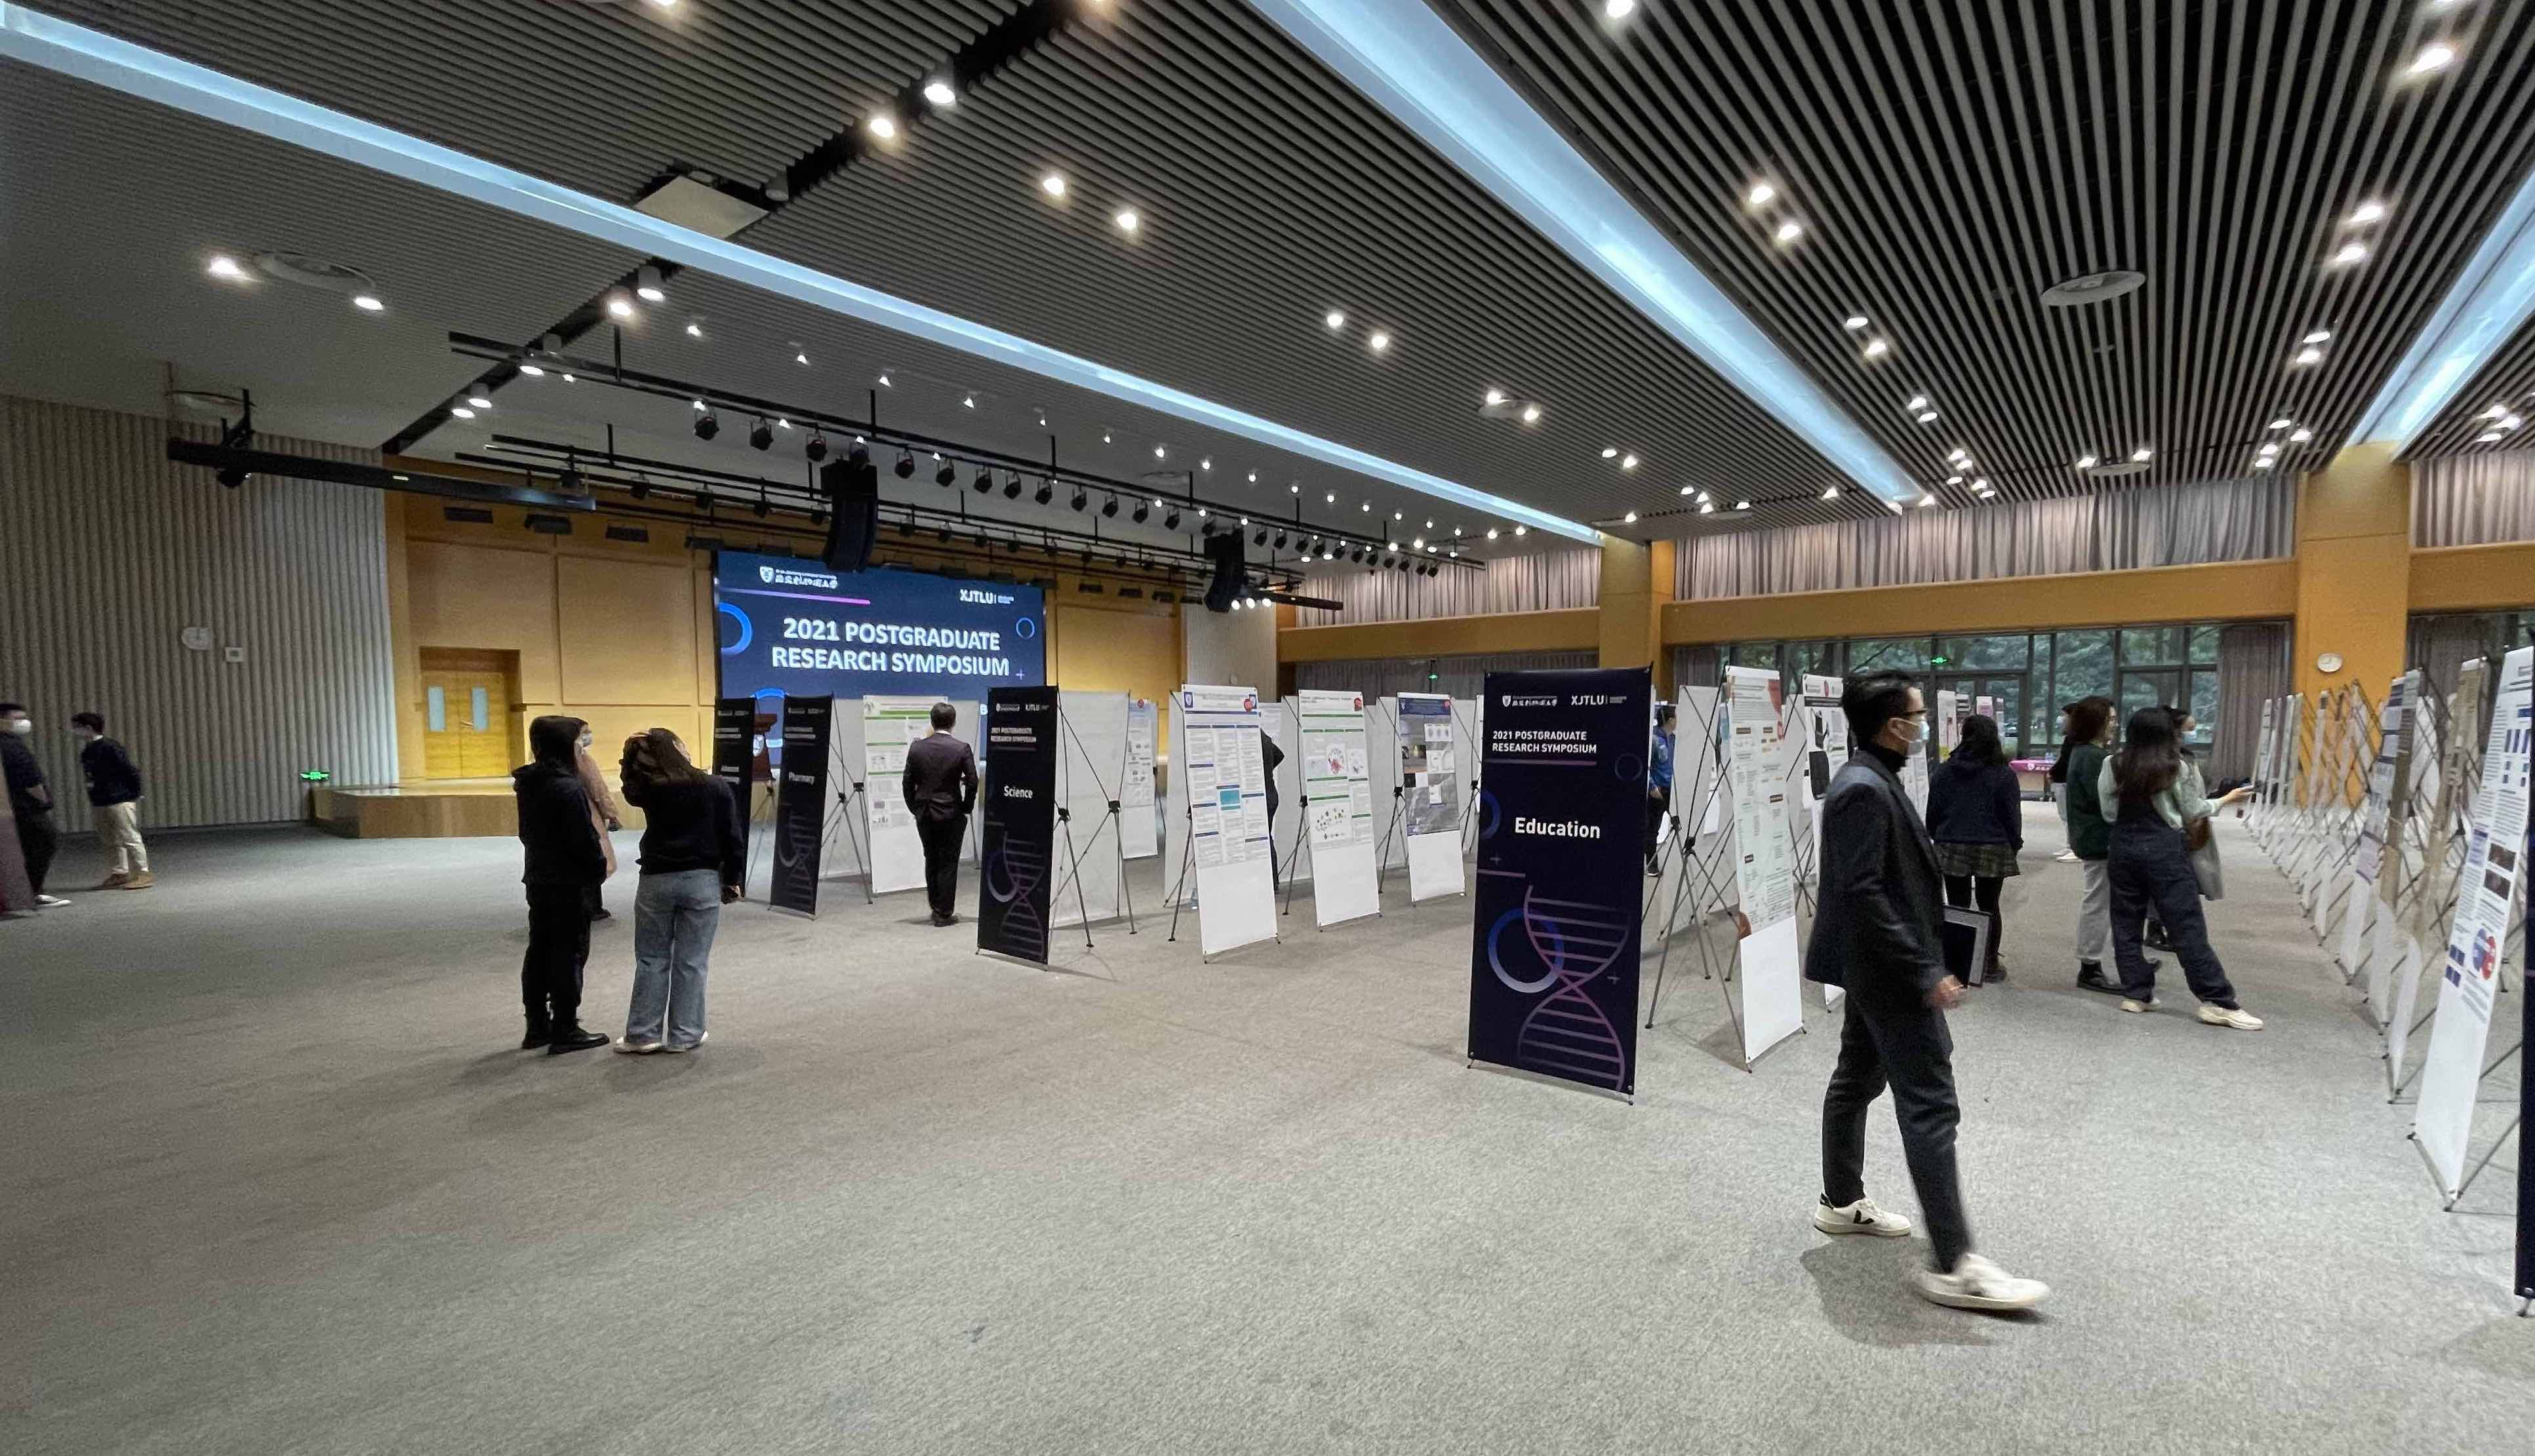
\includegraphics[width=\columnwidth]{author-folder/Kai.Wu/synposium_poster.jpg}
\end{figure}

\subsection{有什么用}

\begin{enumerate}
    \item 锻炼作报告的能力,锻炼你的英语口语。这个展示不会Fail,只会评奖。所以,是很安全的锻炼机会。可不能等到答辩了或者等到你参加顶会了再去锻炼啊。
    \item 可以得奖。学校会请几位老师来听你讲海报、讲PPT,并给你打分。会选出最佳海报奖(10\%)最佳演讲奖(10\%)优秀海报奖(20\%)优秀演讲奖(20\%),会有一张奖状,外加1000和500元的……会议经费(会议经费使用参见章节\ref{section:fund}),虽然不是现金奖励,但还算有用吧\sout{(抠门学校)}。
\end{enumerate}

\subsection{注意事项}

作报告和做海报,大家在网上都能搜到大量教程。但,XPGRS和其他学术报告最大的区别就是,绝大多数同学、包括学校的评审老师,非常有可能完全不知道你的研究领域(正所谓,隔行如隔山)。如果你按照跟你导师汇报的方式来讲,或者是把你在某次内行齐聚的学术会议上的海报/PPT原封不动拿来用,估计是得不了奖的,因为,评委老师和其他同学确实听不懂。

我的导师告诉我,XPGRS因为是给外行讲,和学术报告其实完全不同,更偏向科普性质。如何在短时间内,让一个外行对你的研究感兴趣,并且搞懂个70\%,才是Symposium的目的。如果你不知道该怎么做,可以想象有一天你在电梯里遇到了席酉民,怎么在短时间内让他知道你在做什么,又有什么用,最好还能让他感兴趣。或者是,过年回家跟你哪个亲戚或者老同学怎么讲清楚你在做什么。学术不是闭门造车,如何把自己的学术讲出去,让学术成果造福其他人也是很重要的技能。

\begin{flushright}
(2022年10月19日 by Kai Wu)
\end{flushright}